\documentclass[a4paper,11pt]{article}

\usepackage[utf8]{inputenc}

\usepackage{graphicx}
\usepackage{caption}
\usepackage{subcaption}

\usepackage{pgfplots}
\usepackage{float}
\usepackage{hyperref}
\usepackage{soul}
\hypersetup{
    colorlinks=true, % Enable colored links
    linkcolor=black, % Color for internal links
    urlcolor=black,  % Color for external links
    citecolor=black, % Color for citation links
    pdfborder={0 0 0}, % Remove border around links
}
\newcommand{\underlinehref}[2]{%
    \href{#1}{\ul{#2}}%
}
\pgfplotsset{compat=1.18}


\usepackage{minted}

\begin{document}

    \title{
        \textbf{Sorting Arrays in C}
    }
    \author{Péter Herczku}
    \date{Fall 2024}

    \maketitle

    \section*{Introduction}

    The task is to analyze the time complexity of different sorting algorithms in particular selection, insertion and merge-sort.
    I completed the assignment using the C programming language.

    \section*{Swapping elements in an array}

    Since we will swap elements in multiple algorithms, it's convenient to create a {\tt swap} method that does the job for us.

    \begin{minted}{c}
void swap(int* array, int index1, int index2) {
    int temp = array[index2];
    array[index2] = array[index1];
    array[index1] = temp;
}
    \end{minted}

    \section*{Selection sort}

    The simplest sorting algorithm that is pretty straightforward to implement is selection sort.
    The idea behind it is the following: we start from index 0 and look for the smallest element in the array that is smaller than our value at index 0.
    We swap them, increment index by one, and continue this process until we reach the end of the array.
    In the worst case, we do $n^2/2$ comparisons, therefore this algorithm should have $O(n^2)$ time complexity.
    First, let's take a look at the implementation of selection sort:

    \begin{minted}{c}
void sort(int* array, int length) {
    for (int i = 0; i < length - 1; i++) {
        int candidate = i;
        for(int j = i + 1; j < length; j++) {
            if (array[j] < array[candidate]) {
                candidate = j;
            }
        }
        swap(array, i, candidate);
    }
}
    \end{minted}
    Now, let's run some benchmarks to validate our point about the time complexity of selection sort.

    \begin{figure}[h]
        \centering
        \begin{subfigure}[b]{.5\textwidth}
            \centering
            \includegraphics[width=\textwidth]{./selection/data} % Adjust width or height as needed
        \end{subfigure}
        \caption{Graph of selection sort}
        \label{fig:graph_1}
    \end{figure}

    We can clearly see the quadratic relationship from the graph: if we double the size of the array, the runtime will be multiplied by 4.

    \subsection*{Insertion sort}

    This algorithm is slightly more complex to implement than selection sort, but we still shouldn't have any problems programming it.
    We start from index 1, and we start going backwards.
    If the value of the element at the target index is bigger than our value at the current index we swap them.
    We keep doing this until we reach the beginning of the array, or we reach an element that is smaller than ours.
    After that, we increment index by one and repeat the process until we reach the end of the array.
    Now, let's look at the implementation of the function:

    \begin{minted}{c}
void sort(int* array, int n) {
    for (int i = 1; i < n; i++) {
        for (int j = i - 1; j >= 0 && array[j] > array[j + 1]; j--) {
            swap(array, j, j + 1);
        }
    }
}
    \end{minted}
    In the worst case, it should still be an algorithm with $O(n^2)$ time complexity.
    However, when the array is partially sorted the algorithm should perform better than selection sort.
    After running some benchmarks, we get the following result:

    \begin{figure}[h]
        \centering
        \begin{subfigure}[b]{.5\textwidth}
            \centering
            \includegraphics[width=\textwidth]{./insertion/data} % Adjust width or height as needed
        \end{subfigure}
        \caption{Graph of insertion sort}
        \label{fig:graph_2}
    \end{figure}

    We can observe a quadratic relationship from the graph again.
    Insertion should be theoretically faster than selection sort.
    Let's remove the swap function and implement swapping in-line into our sort function, and run the benchmark again.

    \begin{figure}[h]
        \centering
        \begin{subfigure}[b]{.5\textwidth}
            \centering
            \includegraphics[width=\textwidth]{./insertion_inline/data} % Adjust width or height as needed
        \end{subfigure}
        \caption{Graph of inline insertion sort}
        \label{fig:graph_3}
    \end{figure}

    As we can see we were able to cut back the execution time, but it's till $O(n^2)$.
    Luckily, we can do better.
    Let's discuss it in the next topic.

    \subsection*{Merge sort}

    This algorithm is completely different from the previous ones.
    It's a divide and conquer algorithm, and it divides the array into two halves recursively until each sub array is sorted (contains only one element), then it starts merging them.
    By merging we mean that the algorithm compares the top elements from the array, and put the lower one into the merged array.

    During the division phase, we split the array $log(n)$ times.
    From a geometrical perspective, our runtime rectangle has a length of $n$ and a width of $log(n)$, therefore the time complexity should be $n*log(n)$.

    Since the implementation is too long to include here, you can check it in my GitHub repository, linked at the end of the report.

    After running some benchmarks we got the following results:

    \begin{figure}[H]
        \centering
        \begin{subfigure}[b]{.5\textwidth}
            \centering
            \includegraphics[width=\textwidth]{./merge/data} % Adjust width or height as needed
        \end{subfigure}
        \caption{Graph of merge sort}
        \label{fig:graph_4}
    \end{figure}

    The graph shows a linear like (but not pure linear) relationship, which matches our expected $O(n*log(n))$ time complexity.

    \subsection*{Stability}

    Merge sort is a stable sorting algorithm.
    It means that when there are two elements in the array that are equal, it doesn't rearrange the order of them.
    This is due to the fact that during the merging phase, we always select elements from the left array first.

    \subsection*{Other algorithms}

    It is important to know that there are other algorithms that I did not discuss in this report such as Quicksort.
    This is a sorting algorithm with $O(n*log(n))$ time complexity that has better memory efficiency than merge sort.
    However, it is not a stable sorting algorithm.

    When we are sorting arrays, we cannot just use the algorithm with the best time complexity.
    If we want to insert an element to an array, and we want to keep it sorted, insertion sort will have the best time complexity, and it will outperform merge sort and quicksort.
    When we need to select the smallest elements from an array, selection sort is the optimal choice.
    It is important to be careful when selecting an algorithm, since the best choice highly depends on the use-case.

    \section*{GitHub}
    I have uploaded the full project to \underlinehref{https://github.com/peterherczku/ID1021/tree/main/assignment-4}{my github repository}, where we can find the code used to make this report.

\end{document}
